Since the most important part of our output is on the LCD screen, we recorded only a few screen shots of the serial monitor on PC, for the reason that the serial monitors are only used to check for the correctness of the transmission of commands. For the sake of clarity and convenience, we will show the result in the order of time, or operating logic.
\begin{figure}[!htbp]
	\centering
	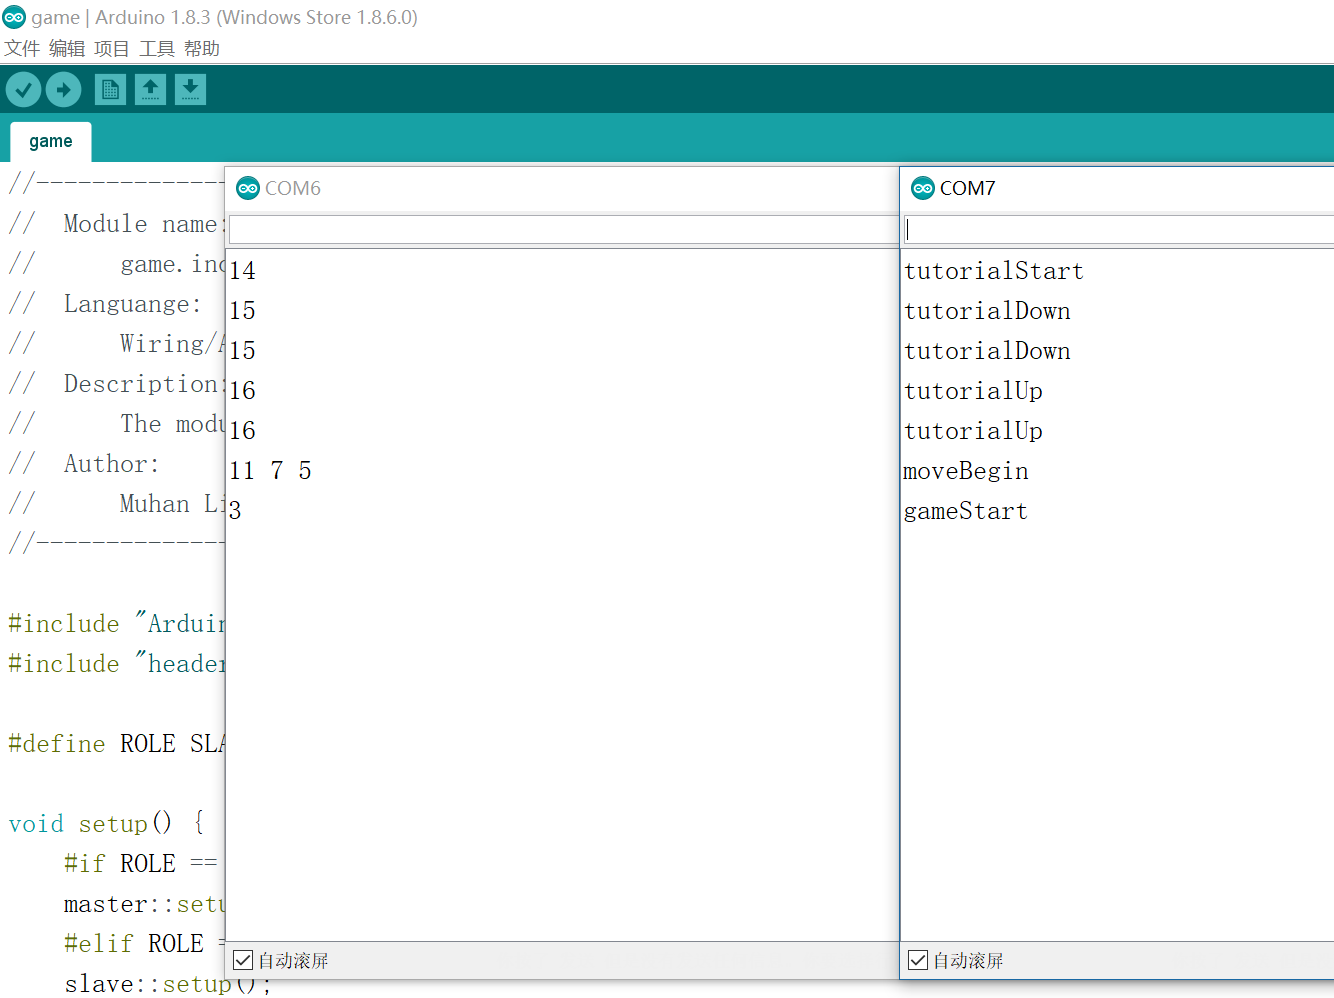
\includegraphics{images/serial.png}
	\caption{The screen shot of serial monitors before the game starts (tutorial page)}
	\label{fig:result}
\end{figure}
\paragraph{Tutorial}
We set the switch of both boards to BOARD after we loaded the modules on the corresponding boards. The serial monitor of the master board shows "14", which represents the start of the tutorial. The following commands meets with the expected results. The serial monitor of the slave board shows "tutorialStart", which indicates that the slave board receive this command and translate it correctly. More details can be found in figure[\ref{fig:result}]. Meanwhile, the LCD screen shows the first page of the tutorial pages. We move the joystick up and down to view all the pages. We push the down button or the right button to leave the tutorial pages.
\paragraph{Setting}
We push the up button to enter the setting page. We can use the joystick to move between the items and change the value of the items. We push the right button to exit the setting page and enter the start game page. In the setting page, the selected item will have left and/or right arrows around the value. The result of the display is the same as expectations.
\paragraph{Game Start}
We only need to move the joystick left and right to choose the box that we want to put something in, and start the game by pressing the right button. The number of boxes displayed on the game start page is correspondent to the number that we set in the setting page. As expected, we can use the joystick to move easily between boxes.
\paragraph{During Game}
After we pressed the right button to confirm the box we choose, the boxes will move to the middle of the screen (vertically)  and switch randomly. The speed and the time of switching depend on the speed and difficulty in the setting page. The boxes switched at an expected speed and repeated for an expected number of times. Then the boxes moved back to second line.
\paragraph{Choose Answer}
After the boxes finishing moving, we pressed the right button to start our choosing. As expected, if we choose the right box, the buzzer will play a happy melody and a heart will come out of the box. It we choose the wrong box, the buzzer will play an angry melody and a cross will come out of the box, then the right answer will be displayed. The first line of the LCD will tell us whether we win or lose. After we press the right button, a new round of game begins.